\chapter{ENHANCEMENT OF MIR-INDUCED HHG BY COHERENT COUPLING WITH THZ FIELD \label{ch:ch5}}

Following a detailed exploration of the phenomenon of dc-current injection and the generation of
population imbalance through the application of two-color linearly polarized laser fields in
Chapter~\ref{ch:ch2}, it is also interesting to explore the enhance or suppress the efficiency of solid-state \gls{HHG} for the development of innovative HHG-based light sources and spectroscopies. Recent investigations have indicated the potential enhancement of HHG from graphene using two-color laser fields explained various mechanisms~\cite{PhysRevB.100.035434,Mrudul:21,PhysRevB.105.195405}.

In the work by Ref.\cite{PhysRevB.100.035434}, the concept of two-color HHG is proposed, involving the interaction of electron-hole pair creation induced by high-frequency pump light and the subsequent acceleration of these created pairs by low-frequency light. Mrudul \textit{et al.} looked into HHG from graphene under bicircular fields, showcasing the ability to control valley polarization\cite{Mrudul:21}. Additionally, Avetissian~\textit{et al.} explored HHG from graphene under linearly polarized light and its second harmonics. They demonstrated that, when the two-color fields are perpendicularly polarized, stronger harmonics can be induced compared to parallel polarization~\cite{PhysRevB.105.195405}.
Recently, \gls{HHG} from graphene has garnered experimental attention in the
mid-infrared (MIR)\cite{doi:10.1126/science.aam8861,cha2022gate} and terahertz
(THz)\cite{Hafez2018,doi:10.1126/sciadv.abf9809} regimes, revealing distinctive ellipticity
dependence and remarkable efficiency. Similar to our previous exploration of HHG from graphene in
the THz regimes in Chapter~\ref{ch:ch4}, based on a quantum master equation, this theoretical methodology has been adeptly applied in the MIR region~\cite{PhysRevB.103.L041408} for the clarification of experimental results~\cite{doi:10.1126/science.aam8861,cha2022gate}.

Furthermore, in the MIR regime, the coupling between field-induced intraband and interband transitions unfolds crucial channels for HHG, leading to enhanced HHG with finite ellipticity~\cite{PhysRevB.103.L041408}. Real-time electron dynamics simulations in the THz regime have highlightd the significance of considering the nonequilibrium steady-state, resulting from the delicate balance between field-driving and relaxation. This approach exceeds the limits of the equilibrium thermodynamic framework and provides a more comprehensive understanding of HHG from graphene~\cite{PhysRevB.106.024313}.

In this chapter, we look into the prospect of adding a terahertz (THz) field to adjust mid-infrared (MIR)-induced \gls{HHG} in graphene, drawing insights from our collective results from previous chapters. Firstly, we employ a quantum master equation to investigate electron dynamics under both MIR and THz fields, subsequently assessing the induced harmonicpectra. The outcomes from fully dynamical calculations are compared with thermodynamic model that incorporates the equilibrium Fermi--Dirac distribution. Additionally, a nonequilibrium population model is considered, justifying a population distribution in a nonequilibrium steady-state. Through our analysis, we reveal the central role played by coupling induced coherence via THz and MIR fields in enhancing MIR-induced HHG. This clarification highlights the significance of field-induced coherence, extending beyond mere population effects.
%=======================================================================================================================================================================
\section{MIR-induced HHG in Graphene under THz Fields}
%=======================================================================================================================================================================
We use the same theoretical model as Chapter.~(\ref{ch:ch4}) by solving quantum master equation as
equation of motion shown in Eq.~(\ref{eqn:masterequation}).
In our analysis of \gls{HHG} induced by a MIR laser pulse in the presence of THz fields, we adopt a practical form for the MIR pulse, expressed as follows:
\begin{align}
	\mathbf A_{MIR}(t) = -\frac{E_{MIR}}{\omega_{MIR}} \mathbf{e}_{MIR}
	\sin(\omega_{MIR} t) \cos^4 \left (\frac{\pi}{T_{MIR}} t \right)
	\label{eqn:laser_pulse}
\end{align}
This pulse is defined in the domain $-T_{MIR}/2<t<T_{MIR}/2$ and is zero outside this range.
Here, $E_{MIR}$ represents the peak strength of the MIR field, $\omega_{MIR}$ is the mean
frequency, $\mathbf e_{MIR}$ is a unit vector indicating the polarization direction of light, and
$T_{MIR}$ is the pulse duration. Specifically, we set the pulse duration $T_{MIR}$ to 0.4 ps and
the mean frequency $\omega_{MIR}$ to 0.35424 eV/$\hbar$ for this study, while other parameters are
varied in our computation.

First, we investigate HHG in graphene only with the MIR fields. For practical analysis, the
direction of the angle $0^\circ$ is fixed to the $\Gamma$--$M$ axis (the $x-$axis in our setup), and the peak field strength of the MIR field $E_{MIR}$ is fixed at 6.5~MV/cm. The induced harmonics are investigated by manipulating the polarization direction of the MIR field, $\mathbf e_{MIR}$.

To analyze the HHG efficiency, we compute the signal intensity of the induced harmonics from
Eq~(\ref{eqn:spectrum})at each
order by integrating the power spectrum within a finite energy range as  the integrated intensity
of the induced $n$th harmonic $I^{n \textrm{th}}_{\mathrm{total}}$:
\begin{align}
	I^{n \textrm{th}}_{\mathrm{total}} = \int_{\left (n-\frac{1}{2} \right )\omega_{MIR}}^{\left (n+\frac{1}{2} \right )\omega_{MIR}} d \omega I_{\textrm{HHG}} (\omega).
	\label{eqn:integrate_intensity}
\end{align}

In the evaluation of the angular dependence of the induced harmonic  $I^{n \textrm{th}}_{\mathrm{total}}$ without THz fields, we analyze the inversion symmetry of graphene. Figures~\ref{fig:SI_polar_mir} illustrate the computed angular dependence of the induced harmonic  $I^{n \textrm{th}}_{\mathrm{total}}$ using only the MIR field. The induced harmonics show a six-fold symmetry, reflecting the hexagonal lattice symmetry of graphene. As showned in Fig.~\ref{fig:SI_polar_mir}, the lower-order harmonics display an almost circular angular dependence, pointing to the circular symmetry in Dirac cones. In contrast, the higher-order harmonics demonstrate a more complicated six-fold symmetry in their angular dependence, owing to the variation of the electronic structure of graphene from a simple Dirac cone when a single-particle energy is distant from the Dirac point.
\begin{figure}[tb]
	\centering
	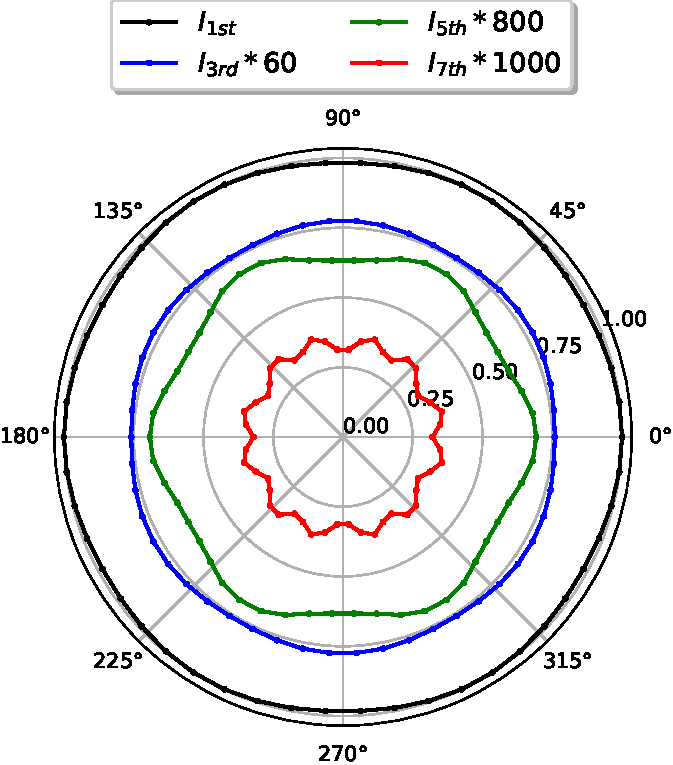
\includegraphics[width=0.50\linewidth]{pic/polar_mir.pdf}
	\caption{\label{fig:SI_polar_mir}
		The angular dependence of the harmonic  obtained from the electron dynamics calculations in the presence of the MIR field. The third, fifth, and seventh harmonic are scaled by factors of 60, 800, and 1000, respectively. Figure is reproduced with permission from ref.~(\cite{PhysRevB.109.045421}). Copyright 2024, Phys. Rev. B.
	}
\end{figure}
Similarly, we adopt the subsequent expression for the THz pulse:
\begin{align}
	\mathbf A_{THz}(t) = -\frac{E_{THz}}{\omega_{THz}} \mathbf{e}{THz}
	\sin(\omega{THz} t) \cos^4 \left (\frac{\pi}{T_{THz}} t \right)
	\label{eqn:laser_pulse}
\end{align}
within the period $-T_{THz}/2 < t < T_{THz}/2$, and zero outside this range. Here, $E_{THz}$ denotes the peak strength of the THz field, $\omega_{THz}$ is the mean frequency, $\mathbf e_{THz}$ represents a unit vector along the polarization direction, and $T_{THz}$ stands for the pulse duration. In our investigation, the pulse duration $T_{THz}$ is fixed at 40 ps, and the mean frequency $\omega_{THz}$ is set to 1.2407 meV/$\hbar$. The time profile of the applied THz electric field is showned in Fig.\ref{fig:current}(a).

To illuminate the complexity of THz-assisted MIR-induced \gls{HHG} in graphene, we conduct an electron dynamics calculation in the presence of both THz and MIR fields, denoted as $\mathbf E_{THz}(t) + \mathbf E_{MIR}(t)$. Here, we set $E_{MIR}$ to 6.5 MV/cm and $E_{THz}$ to 0.5 MV/cm. It is appropriate to note that experimentally available intense THz pulses can show amplitudes exceeding 1 MV/cm~\cite{10.1063/1.3560062}. The polarization direction of the THz field $\mathbf e_{THz}$ is $\Gamma$--$M$ direction (the $x$-direction in our setup), while the polarization direction of the MIR field $\mathbf e_{MIR}$ is considered as a tunable parameter. Figures~\ref{fig:current}(a) and (b) illustrate the computed current $\mathbf J(t)$ induced by $\mathbf E_{THz}(t) + \mathbf E_{MIR}(t)$ as a function of time. The result for the parallel configuration ($\mathbf e_{MIR} = \mathbf e_x = \mathbf e_{THz}$) is presented in Fig.\ref{fig:current}(a), while the result for the perpendicular configuration ($\mathbf e_{MIR} = \mathbf e_y \perp \mathbf e_{THz}$) is shown in Fig.\ref{fig:current}(b). The $x$ and $y$ components are represented by blue and red lines, respectively. Evidently, Figs.\ref{fig:current}~(a) and (b) illustrate that the THz field induces a current on the picosecond time scale, whereas the MIR field induces a current on a much shorter time scale.
\begin{figure*}[ht]
	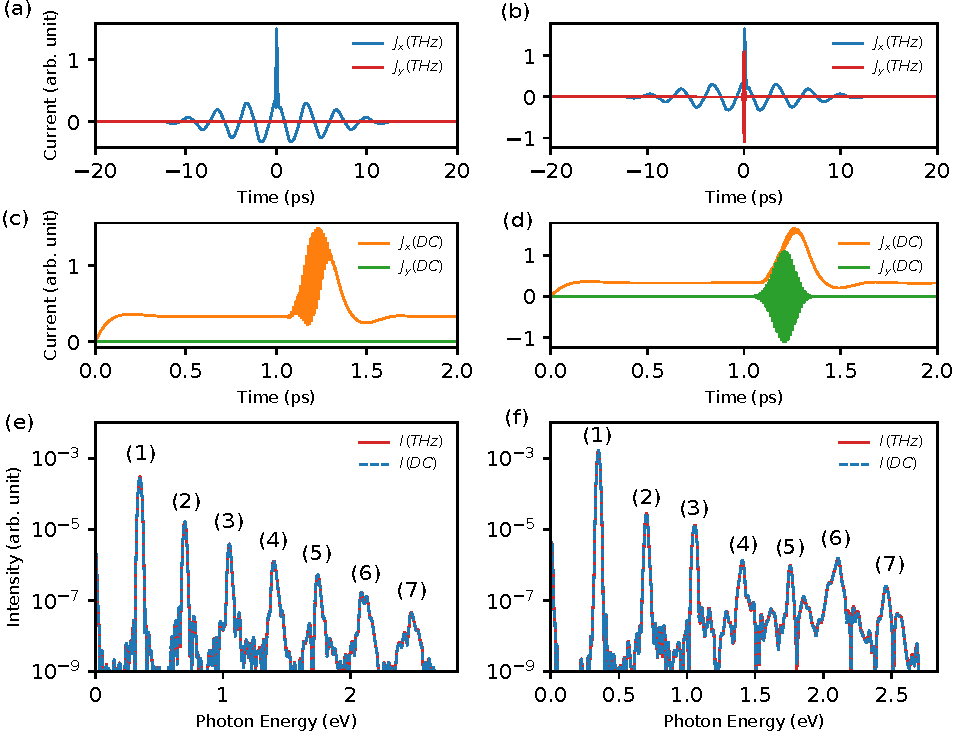
\includegraphics[width=0.9\linewidth]{pic/fig1.pdf}
	\caption{\label{fig:current}
		(a, b)~The current $\mathbf{J} (t)$ induced by THz and MIR fields, $\mathbf E_{THz}(t)+\mathbf E_{MIR}(t)$. The $x$-component of the current is shown as the blue line, whereas the $y$-component is shown as the red line. Panel (a) shows the time profile of the applied THz field. (c, d)~The current $\mathbf{J}(t)$ induced by the static and MIR fields, $\mathbf E_{dc}(t)+\mathbf E_{MIR}(t-\tau_{MIR})$. The $x$ component of the current is shown as the orange line, whereas the $y$-component is shown as the green line. In the panels~(a) and (c), the polarization of all the fields is parallel to the $\Gamma$--$M$ direction (the $x$-direction in the present setup) as $\mathbf e_{THz}=\mathbf e_{dc}=\mathbf e_{MIR}=\mathbf e_x$. In the panels~(b) and (d), the polarization of THz and static fields is parallel to the $x$-direction as $\mathbf e_{THz}=\mathbf e_{dc}=\mathbf e_{MIR}=\mathbf e_x$, while that of the MIR field is perpendicular as $\mathbf e_{MIR}=\mathbf e_y$. (e) The power spectra $I_{\mathrm{HHG}}(\omega)$ computed using the current in (a) and (c). (f) The power spectra $I_{\mathrm{HHG}}(\omega)$ computed using the current in (b) and (d). Panels are reproduced with permission from ref.~(\cite{PhysRevB.109.045421}). Copyright 2024, Phys. Rev. B.
	}
\end{figure*}

To look into MIR-induced \gls{HHG} with the presence of THz fields, we investigate the current induced by the MIR field under the influence of the THz field. For this analysis, we compute two types of currents. Firstly, we denote the current induced by both the THz and MIR fields as $\mathbf J^{THz + MIR}(t)$. Secondly, we denote the current induced solely by the THz field as $\mathbf J^{THz}(t)$. Defining the current induced by the MIR field in the presence of the THz field as $\mathbf J^{eff}(t) = \mathbf J^{THz + MIR}(t) - \mathbf J^{THz}(t)$, we subject it to Fourier transformation, followed by computation of the power spectrum of the induced harmonics using Eq.(\ref{eqn:spectrum}). The solid line in Fig.\ref{fig:current}(e) shows the power spectrum computed using the current $\mathbf J(t)$ showned in Fig.\ref{fig:current}(a), where the polarization directions of the THz and MIR fields are parallel. On the other hand, the solid line in Fig.\ref{fig:current}(f) shows the power spectrum computed employing the current $\mathbf J(t)$ illustrated in Fig.\ref{fig:current}(b), where the polarization directions of the two fields are perpendicular. Notably, Fig.\ref{fig:current}(e) illustrates the generation of second and higher even-order harmonics next to odd-order harmonics, attributed to the local breakdown of the system's inversion symmetry induced by the THz field. This phenomenon, known as electric-field-induced second-harmonic generation (EFISH) or THz-induced second-harmonic generation (TFISH), has been extensively studied\cite{PhysRevLett.8.404,PhysRev.137.A801,Nahata:98,COOK1999221}. Similarly, even-order harmonics are generated in the perpendicular configuration ($\mathbf e_{MIR} \perp \mathbf e_{THz}$), as showned in Fig.\ref{fig:current}(f).

Including the THz pulse in the electron dynamics computation extends the propagation time (42 ps in the current situation), as illustrated in Figs.\ref{fig:current}(a) and (b). Consequently, performing electron dynamics calculations with the obvious inclusion of THz pulses involves a substantial computational trouble. To alleviate the computational overhead associated with modeling MIR-induced \gls{HHG} in graphene under a THz field, we adopt a static field approximation based on the quasi-static approximation described in Chapter~\ref{ch:ch4}.

For practical analysis, we conduct two simulations. In the first simulation, electron dynamics are computed under a static field $\mathbf E_{dc}(t) = \mathbf e_{dc} E_{dc}\Theta(t)$, suddenly initiated at $t=0$. Here, $\mathbf e_{dc}$ represents the unit vector along the polarization direction of the static field, and $E_{dc}$ denotes the field strength. Upon the sudden activation of the static field, the induced electron dynamics prompt a current. Following a sufficiently long time of propagation, the driven system attains a steady state, and the current stabilizes over time. We designate the current induced solely by $\mathbf E_{dc}(t)$ as $\mathbf J^{dc}(t)$.

In the second simulation, electron dynamics are computed under both the MIR and static fields, $\mathbf E_{dc}(t) + \mathbf E_{MIR}(t - \tau_{MIR})$, where the pulse center of the MIR field is shifted by $\tau_{MIR}$. We denote the current induced by $\mathbf E_{dc}(t) + \mathbf E_{MIR}(t - \tau_{MIR})$ as $\mathbf J^{dc+MIR}(t)$. The shift $\tau_{MIR}$ can be made sufficiently large to investigate the MIR-induced electron dynamics for a full nonequilibrium steady state realized by the static field $\mathbf E_{dc}(t)$. Subsequently, the MIR-induced current can be extracted as $\mathbf J^{eff}(t) = \mathbf J^{dc+MIR}(t) - \mathbf J^{dc}(t)$ to analyze MIR-induced HHG in the presence of the static field.

Figures~\ref{fig:current}(c) and (d) illustrate the current $\mathbf J^{dc+MIR}(t)$ induced by both the static and MIR fields. The orange and green lines represent the $x$ and $y$ components of the current, respectively. Here, the static field along the $\Gamma$--$M$ direction (the $x$-direction in our setup), and its strength $E_{dc}$ matches the peak strength of the THz field, $E_{dc}=E_{THz}=0.5$MV/cm. In Fig.\ref{fig:current}(c), the MIR field aligns parallel to the static field, while in Fig.\ref{fig:current}(d), it is perpendicular to the static field. To incorporate the MIR field into the nonequilibrium steady-state under the static field, we set the time delay $\tau_{MIR}$ of the MIR field to 1~ps, exceeding the relaxation time scales of the quantum master equation, $T_1$ and $T_2$.

To investigate HHG in the presence of the static field $\mathbf E_{dc}(t)$, we extract the current
$\mathbf J^{eff}(t)$ induced by the MIR field in the presence of the static field by subtracting
$\mathbf J^{dc}(t)$ from $\mathbf J^{dc+MIR}(t)$: $\mathbf J^{eff}(t)=\mathbf J^{dc+MIR}(t)-\mathbf
	J^{dc}(t)$. The dashed lines in Figs~\ref{fig:current}(e) and (f) represent the HHG spectra
computed using the current shown in Figs\ref{fig:current}(c) and (d), respectively. Remarkably, the
results obtained through the quasi-static approximation with a static field align perfectly with
those computed by obviously including the THz pulse. This consistency highlights the validity of
the quasi-static approximation for analyzing HHG under MIR and THz fields. Additionally, we verified
the consistency of the quasi-static approximation across various static field strengths (refer to
Figure~\ref{fig:SI_polar_mir}). Hereafter, we employ the static field within the quasi-static approximation rather than obviously including the THz pulse.

\begin{figure}[tb]
	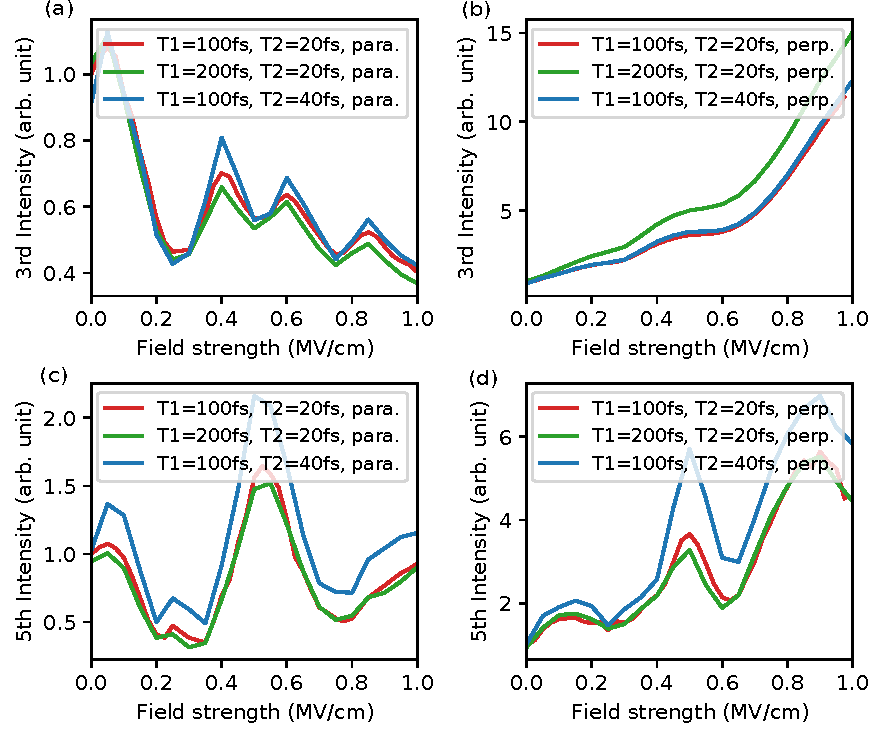
\includegraphics[width=0.9\linewidth]{pic/SI_t1t2.pdf}
	\caption{\label{fig:intensity_relaxation}
		The harmonic are shown as a function of the static field strength $E_{dc}$. In each panel, the results obtained using the different relaxation times, $T_1$ and $T_2$, are compared. The results of the third harmonics are shown in the panels~(a) and (b), whereas those of the fifth harmonics are shown in the panels~(c) and (d). The results obtained using the parallel configuration ($\mathbf e_{MIR}=\mathbf e_x = \mathbf e_{THz}$) are shown in the panels~(a) and (c), whereas those obtained using the perpendicular configuration ($\mathbf e_{MIR}=\mathbf e_y \perp \mathbf e_{THz}$) are shown in the panels~(b) and (d). Panels are reproduced with permission from ref.~(\cite{PhysRevB.109.045421}). Copyright 2024, Phys. Rev. B.
	}
\end{figure}

We further investigate the influence of relaxation times, $T_1$ and $T_2$, on HHG in the presence
of THz and MIR fields. Employing the methods outlined in Section.~\ref{sec:master}, we compute the intensity of third- and fifth-order harmonics under varying relaxation times. The results, showned in Fig.\ref{fig:intensity_relaxation}, show consistent qualitative trends in HHG enhancement with THz field irradiation across different relaxation times. Thus, the specific choice of relaxation times does not substantially change the enhancement phenomenon.

Relaxation times are determined by diverse scattering mechanisms, including electron-electron,
electron-phonon, and electron-impurity interactions. Consequently, the actual relaxation times in
practical settings depend on experimental conditions. Nonetheless, the findings presented in
Fig.~\ref{fig:intensity_relaxation} suggest that HHG enhancement via THz field irradiation can
present as a robust phenomenon across a broad spectrum of experimental situations.

\begin{figure}[tb]
	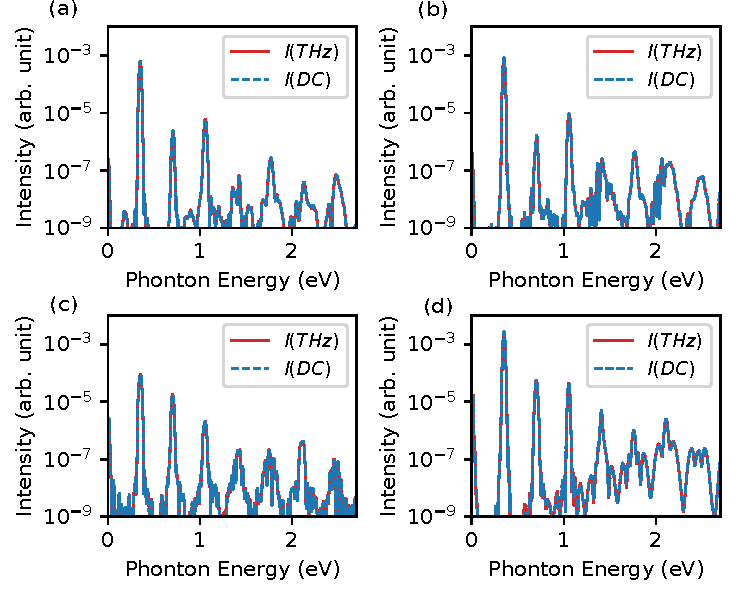
\includegraphics[width=0.9\linewidth]{pic/SI_hhg.pdf}
	\caption{\label{fig:quasi-static}
		The power spectra of induced harmonics, $I_{HHG}(\omega)$, are shown. The results obtained using a weak THz field ($E_{THz}=0.1$~MV/cm) are shown in the panels~(a) and (b), while those obtained using a strong THz field ($E_{THz}=1.0$~MV/cm) are shown in the panels~(c) and (d). The results obtained using the parallel configuration ($\mathbf e_{MIR}=\mathbf e_x = \mathbf e_{THz}$) are shown in the panels~(a) and (c), whereas those obtained using the perpendicular configuration ($\mathbf e_{MIR}=\mathbf e_y \perp \mathbf e_{THz}$) are shown in the panels~(b) and (d). Panels are reproduced with permission from ref.~(\cite{PhysRevB.109.045421}). Copyright 2024, Phys. Rev. B.
	}
\end{figure}

We extend our investigation to validate the quasi-static approximation across varying strengths of the THz field. We repeat the analyses presented in Figs.\ref{fig:current}(e) and (f) while changeing the THz field strength. Results obtained under a weak THz field ($E_{THz}=0.1$MV/cm) are showned in Figs.\ref{fig:quasi-static}(a) and (b), while those under a strong THz field ($E_{THz}=1.0$MV/cm) are shown in Figs.\ref{fig:quasi-static}(c) and (d). As observed from the figures, the outcomes of the quasi-static approximation closely reflect those obtained from calculations with THz laser pulses across all investigated field strengths and polarization directions. Hence, we affirm the efficacy of the quasi-static approximation in accurately describing electron dynamics in graphene under THz and MIR fields, encompassing both weak and strong field regimes.
This agreement between the quasi-static approximation and the obvious inclusion of the THz pulse highlights the central role played by the nonequilibrium steady state under the static field in MIR-induced HHG in graphene in the presence of a THz field.
%=======================================================================================================================================================================
\section{Orientational Dependence of HHG}
%=======================================================================================================================================================================
\begin{figure*}[tp]
	\centering
	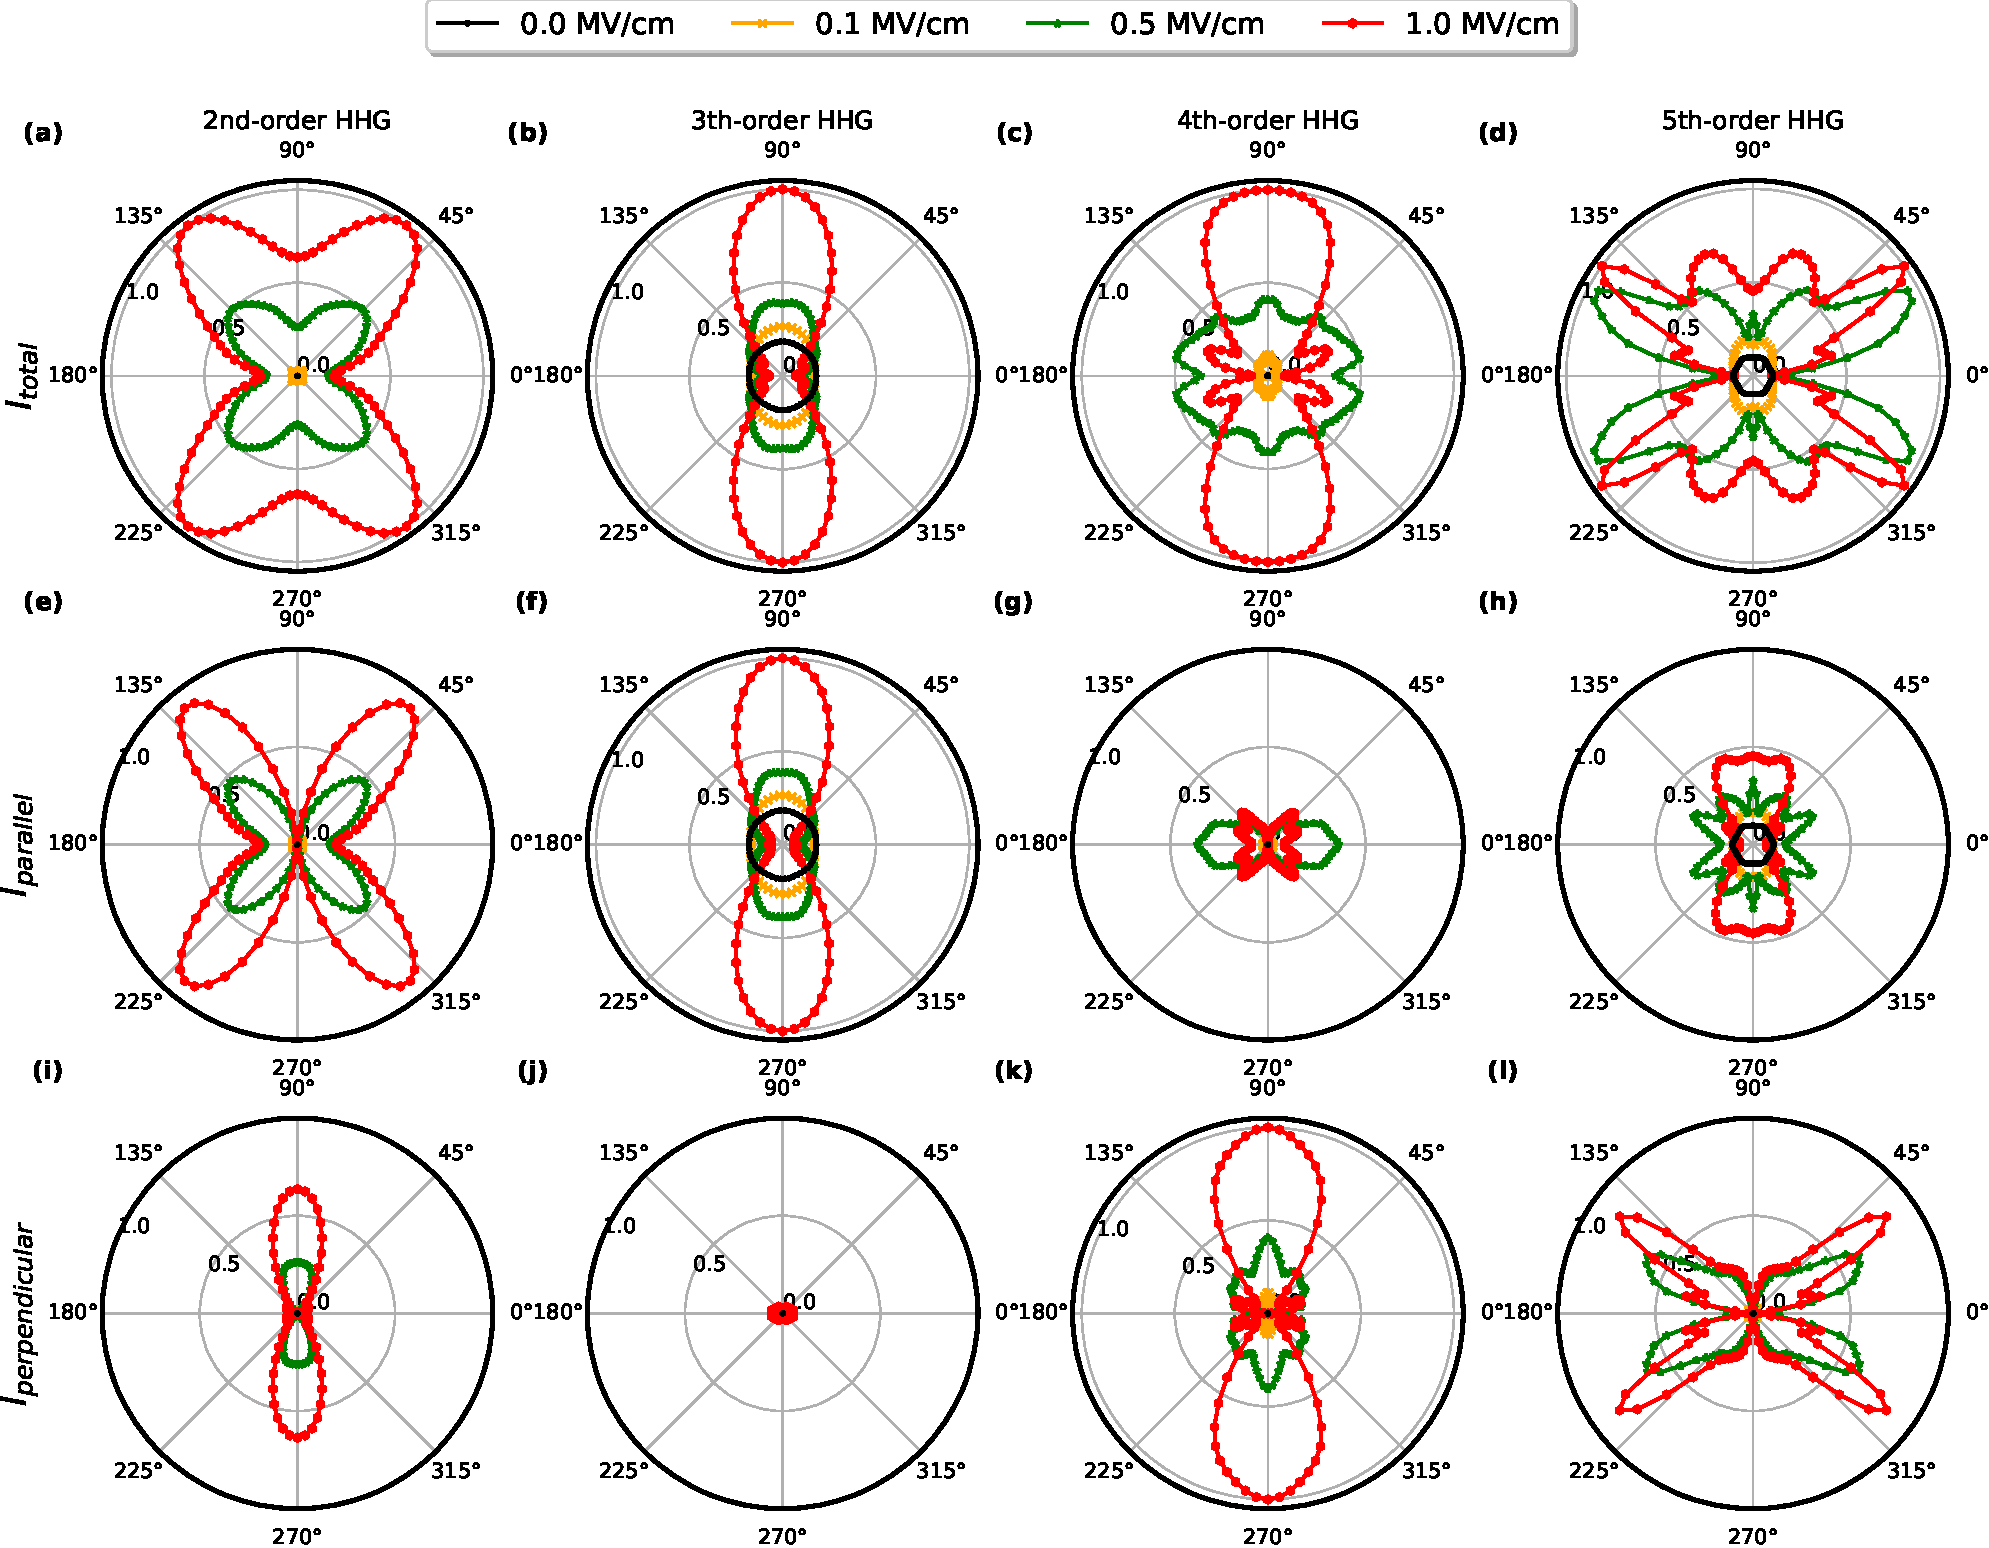
\includegraphics[width=1.0\linewidth]{pic/polar.pdf}
	\caption{
		% The angular dependence of the harmonic  in the nonequilibrium steady-states under a static field along the $\Gamma$--$M$ direction is shown for different static field strengths, $E_{dc}$. The angle $\theta$ denotes the relative angle between the static field and the $MIR$ field. (a--d) The total intensity $I^{n \textrm{th}}_{\mathrm{total}}$ is shown for the second, third, fourth, and fifth harmonics. (e-h) The component of the intensity parallel to $\mathbf e_{MIR}$ is shown for each harmonic. (i-l) The component of the intensity perpendicular to $\mathbf e_{MIR}$ is shown for each harmonic. The results are normalized by the maximum total intensity $I^{n \textrm{th}}_{\mathrm{total}}$ for each harmonic. Panels are reproduced with permission from ref.~(\cite{PhysRevB.109.045421}). Copyright 2024, Phys. Rev. B.
	}\label{fig:polar}
\end{figure*}

We explore high-harmonic generation (HHG) in graphene within the quasi-static approximation, varying the relative angle between the static and MIR fields. For our analysis, we maintain the direction of the static field $\mathbf e_{dc}$ along the $\Gamma$--$M$ axis (the $x$-axis in our setup) and set the peak field strength of the MIR field $E_{MIR}$ to 6.5~MV/cm. We investigate the induced harmonics by manipulating the polarization direction of the MIR field, $\mathbf e_{MIR}$, and adjusting the strength of the static field, $E_{dc}$.

Figures~\ref{fig:polar}(a--d) illustrate the angular dependence of the induced harmonic  $I^{n \textrm{th}}$ for various harmonic orders. Here, $\theta$ represents the relative angle between the MIR and static fields. In Fig.\ref{fig:polar}(a), absence of a static field results in no second harmonic generation, given the inversion symmetry of graphene. However, with the introduction of a static field, second harmonics emerge due to the breakdown of this symmetry. Notably, for a static field strength of 0.5MV/cm, the induced second-harmonic intensity peaks at approximately 45$^{\circ}$ relative angle.

In Fig.\ref{fig:polar}(b), the third-harmonic  appears nearly isotropic (showned by the black
line) in the absence of a static field, reflecting the rotational symmetry of the Dirac cone (refer
also to Figure~\ref{fig:SI_polar_mir}). On the other hand, under the influence of a strong static field ($E_{dc}=1.0$MV/cm), the third-harmonic intensity shows significant angular dependence: it is notably enhanced when the static and MIR fields are perpendicular to each other, whereas it is suppressed for parallel field orientations. This enhancement for the perpendicular configuration can be attributed to the coupling between the intraband transition induced by the static field and the interband transition induced by the MIR field, as previously suggested\cite{PhysRevB.103.L041408}.

The angular dependence of higher-order harmonics becomes more complicated under a static field, as
showned in Figs.\ref{fig:polar}(c) and (d). Notably, the fifth-order harmonic emission shows
significant enhancement in the presence of either static or THz fields (Fig.\ref{fig:polar}(d)).
For instance, applying a static field of 0.5MV/cm boosts the fifth-order harmonic intensity by more
than tenfold compared to that induced solely by the MIR field (indicated by the green line in
Fig.\ref{fig:polar}(d)). This enhancement ratio surpasses that observed for the third-order
harmonic, suggesting a greater potential for field-induced enhancement in higher-order harmonics.
Indeed, the seventh-order harmonichows a 25-fold enhancement with a static field strength of
0.5MV/cm (refer to Figure~\ref{fig:SI_polar_mir}).

To further illustrate the angular dependence of HHG in graphene, we decompose the harmonic intensity $I_{\mathrm{HHG}}(\omega)$ into parallel and perpendicular components with respect to the polarization of the driving MIR field. The parallel component of the HHG intensity is defined as
\begin{align}
	I^{\textrm{para}}_{\mathrm{HHG}}(\omega)\sim \omega^2 \left | \int^{\infty}_{-\infty} dt \mathbf e_{MIR} \cdot \mathbf J(t) e^{i\omega t} \right |^2,
	\label{eqn:spectrum-para}
\end{align}
where $\mathbf e_{MIR}$ is the unit vector along the polarization direction of the MIR field. Likewise, the perpendicular component is defined as
\begin{align}
	I^{\textrm{perp}}_{\mathrm{HHG}}(\omega)\sim \omega^2 \left | \int^{\infty}_{-\infty} dt \bar{\mathbf e}_{MIR} \cdot \mathbf J(t) e^{i\omega t} \right |^2,
	\label{eqn:spectrum-perp}
\end{align}
where $\bar{\mathbf e}_{MIR}$ is a unit vector perpendicular to $\mathbf e_{MIR}$, i.e., $\bar{\mathbf e}_{MIR} \cdot\mathbf e_{MIR}=0$. The total intensity $I_{\textrm{HHG}}$ in Eq.~(\ref{eqn:spectrum}) is reproduced by the sum of $I^{\textrm{para}}_{\mathrm{HHG}}(\omega)$ and $I^{\textrm{perp}}_{\mathrm{HHG}}(\omega)$ as $I_{\mathrm{HHG}}(\omega)=I^{\textrm{para}}_{\mathrm{HHG}}(\omega)+I^{\textrm{perp}}_{\mathrm{HHG}}(\omega)$.

Equations (\ref{eqn:spectrum-para}) and (\ref{eqn:spectrum-perp}) are used to separate the induced harmonic intensity into parallel and perpendicular components. Figures~\ref{fig:polar}~(e--h) and (i--l) illustrate the angular dependence of the parallel and perpendicular components of the harmonic intensity, respectively, for different orders.

In Figs.\ref{fig:polar}(a), (e), and (i), the parallel component of the second harmonic under the static field peaks around 45$^{\circ}$, constituting the dominant contribution to the total second-harmonic intensity at this orientation. On the other hand, the maximum perpendicular component is consistently achieved when the MIR and static fields are orthogonal to each other. In Figs.\ref{fig:polar}(b), (f), and (j), the third harmonic is predominantly governed by its parallel component across all angles and static field strengths examined. Notably, for both second- and third-harmonic generation, the parallel components prevail when the induced harmonic intensity is maximized.

Qualitative distinctions emerge between the lower-order harmonics (second and third) and the
higher-order ones (fourth and fifth). In Fig.\ref{fig:polar}(c), the fourth harmonic  peaks at
an angle $\theta$ of 90$^{\circ}$ under the strongest applied static field, $E_{dc}=1.0$MV/cm. A
comparison of Figs.\ref{fig:polar}(g) and (k) reveals the predominance of the perpendicular
component in the induced harmonic intensity under these conditions. On the other hand, as showned in
Figs.\ref{fig:polar}(d), (h), and (l), the induced fifth harmonic at the most efficient angle is
primarily governed by the perpendicular component, despite the dominance of the parallel component
at all angles in the absence of a static field. Hence, the emission pathways associated with the
perpendicular components are expected to play a crucial role in enhancing MIR-induced HHG by a
THz field. This trend persists for higher-order harmonics as well (see Figure\ref{fig:SI_polar}):
\begin{figure}[hbp]
	\center
	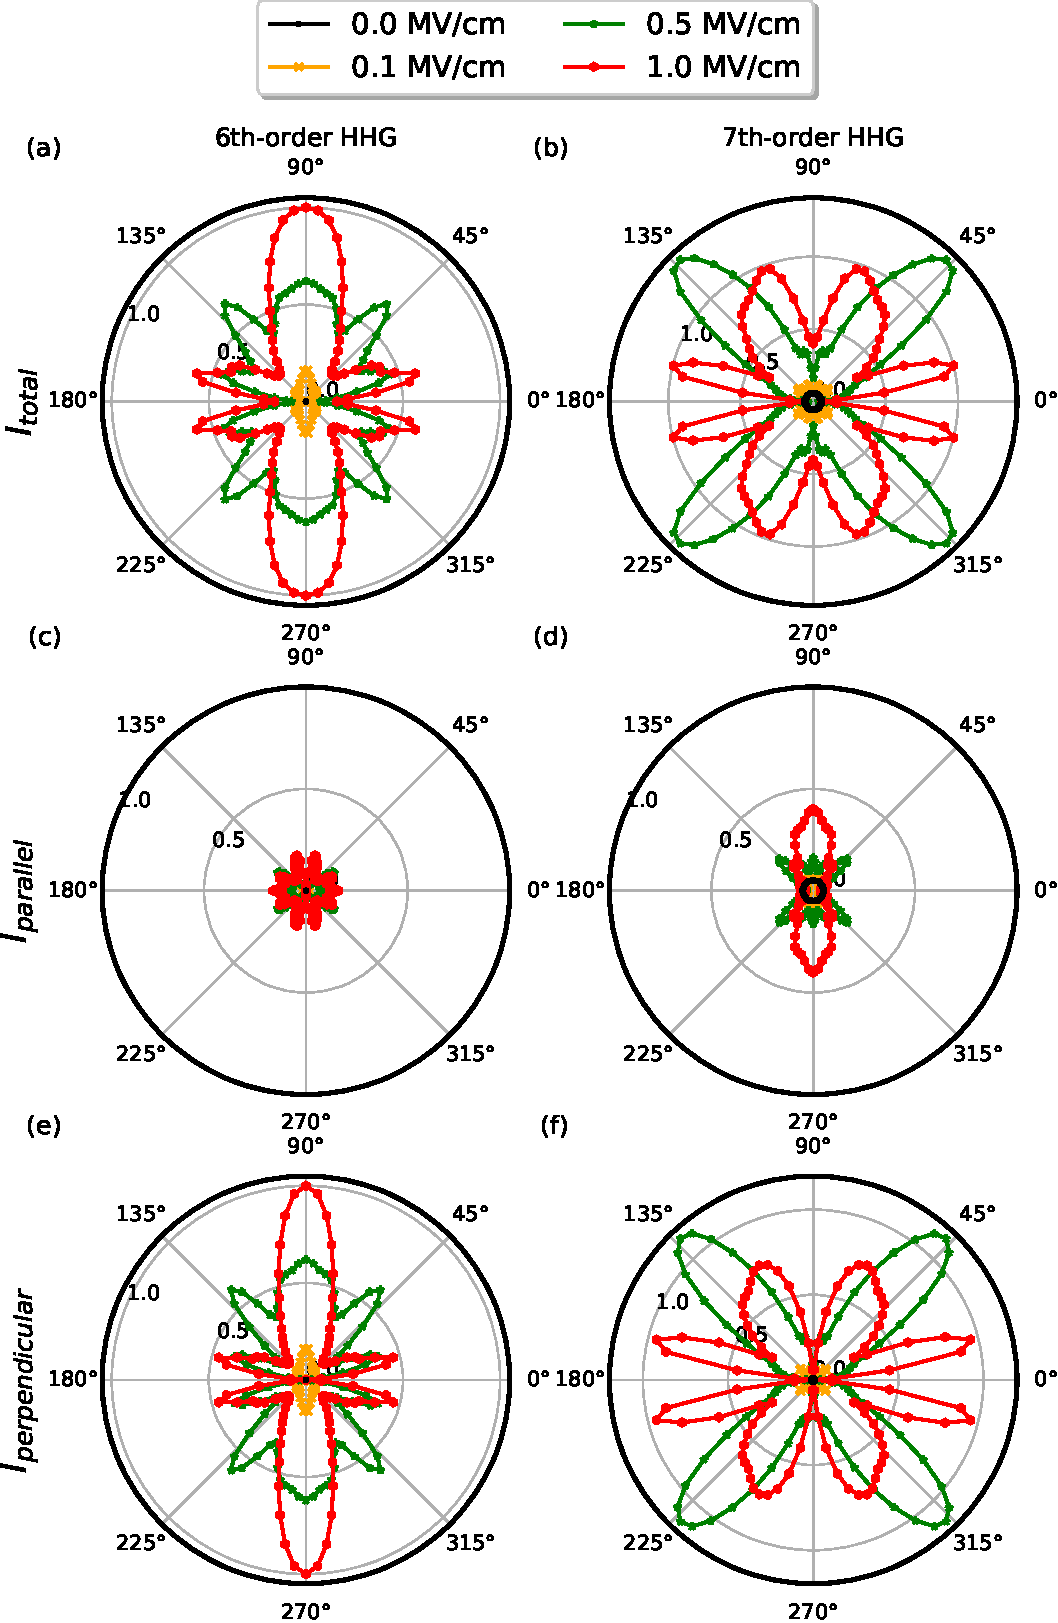
\includegraphics[width=0.8\linewidth]{pic/SI_polar.pdf}
	\caption{\label{fig:SI_polar}
		The angular dependence of the harmonic yields in the nonequilibrium steady state under a static field along the $\Gamma$--$M$ direction is shown. The angle $\theta$ denotes the relative angle between the static field and the $MIR$ field. (a and b) The total intensity $I^{n \textrm{th}}_{\mathrm{total}}$ for the sixth and seventh harmonics is shown, respectively. (c and d) The component of the intensity parallel to $\vecb e_{MIR}$ is shown for each harmonic. (e and h) Th component of the intensity perpendicular to $\vecb e_{MIR}$ is shown for each harmonic. The results are normalized by the maximum total intensity $I^{n \textrm{th}}_{\mathrm{total}}$ of each harmonic. Panels are reproduced with permission from ref.~(\cite{PhysRevB.109.045421}). Copyright 2024, Phys. Rev. B.
	}
\end{figure}
The angular dependency of the 6th(Figures\ref{fig:SI_polar}(a)) and 7th (Figures\ref{fig:SI_polar}(b)) \gls{HHG} is analyzed similarly to the approach used in Fig.\ref{fig:polar}. Further examination reveals in Figs.\ref{fig:SI_polar}(c) and (e) the decomposition of the sixth-harmonic signal into parallel and perpendicular components, while the same analysis is conducted for the seventh-order harmonic in Figs.\ref{fig:SI_polar}(d) and (f). In accordance with the findings for the fourth and fifth harmonics illustrated in Fig.\ref{fig:polar}, it is evident from Fig.~\ref{fig:SI_polar} that the perpendicular components play a significant role in the enhancement of mid-infrared (MIR)-induced high harmonic generation (HHG) by a terahertz (THz) field.

%=======================================================================================================================================================================
\section{Comparison of Nonequilibrium Steady State and Thermodynamic Model}
%=======================================================================================================================================================================
\begin{figure}[htp]
	\center
	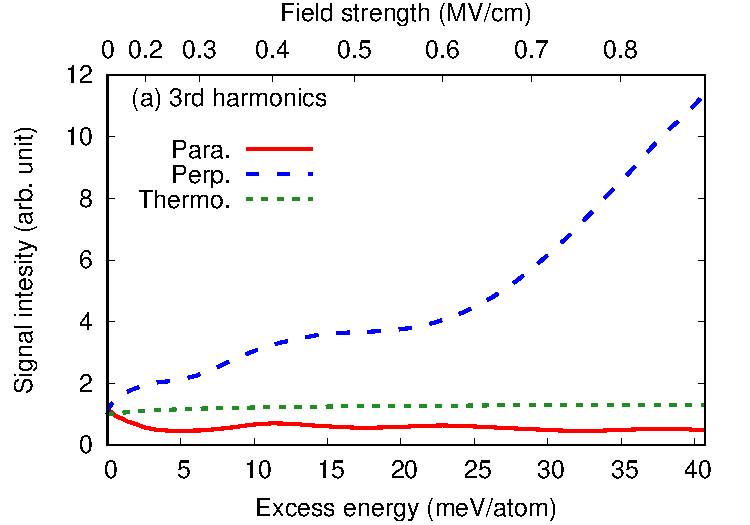
\includegraphics[width=0.7\linewidth]{pic/3rd_hh_vs_thermal.pdf}
	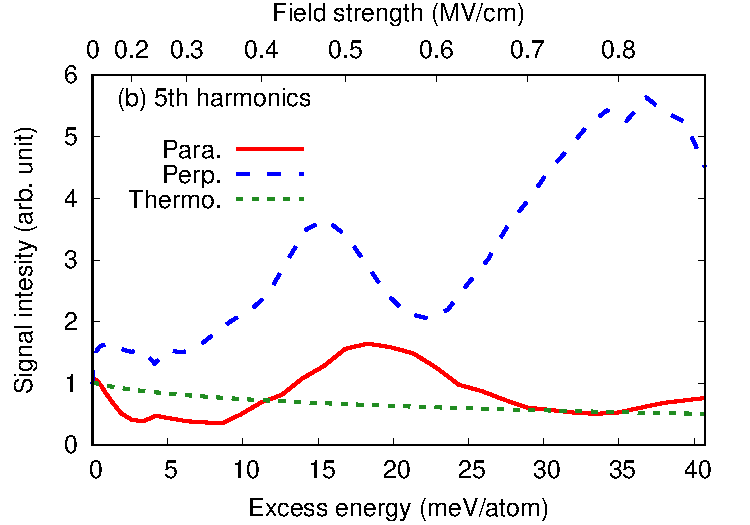
\includegraphics[width=0.7\linewidth]{pic/5th_hh_vs_thermal.pdf}
	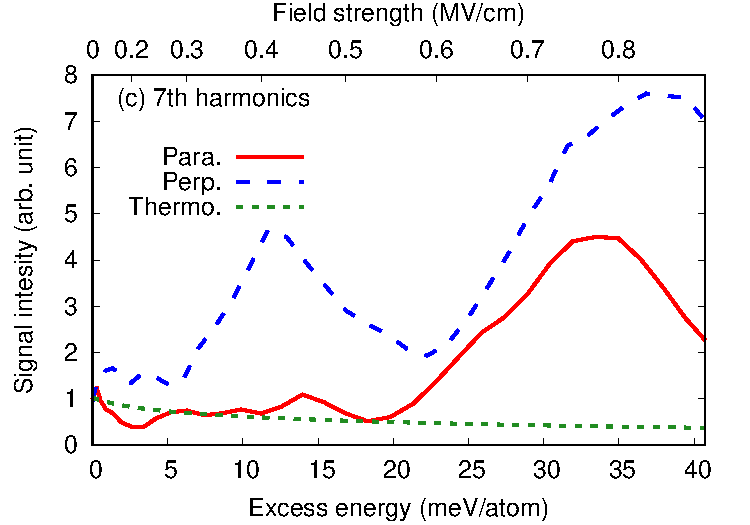
\includegraphics[width=0.7\linewidth]{pic/7th_hh_vs_thermal.pdf}
	\caption{\label{fig:intensity_tem}
		The induced light intensity, $I^{\textit{n}th}$, is shown as a function of the excess energy for (a) third (b) fifth, and (c) seventh harmonics. The results for the nonequilibrium steady-states induced by a static field parallel (red solid line) and perpendicular (blue dashed line) to the MIR field are compared with the thermodynamic model (green dotted line). In each panel, the field strength of the static field parallel to the MIR field is shown as the secondary axis. Panels are reproduced with permission from ref.~(\cite{PhysRevB.109.045421}). Copyright 2024, Phys. Rev. B. Panels are reproduced with permission from ref.~(\cite{PhysRevB.109.045421}). Copyright 2024, Phys. Rev. B.
	}
\end{figure}

In this investigation, we look into the role of nonequilibrium steady states in high harmonic generation (HHG) by comparing the outcomes of the quasi-static approximation with those derived from the thermodynamic model~\cite{mics2015thermodynamic}, a framework previously used in studying HHG in graphene under THz fields~\cite{Hafez2018,doi:10.1126/sciadv.abf9809}. The quasi-static approximation replaces the THz pulse with a static field to describe the electronic system's behavior under THz irradiation, whereas the thermodynamic model approximates the system's response to a THz pulse as a high-temperature thermal state~\cite{mics2015thermodynamic}. The difference between these models illustrates the influence of nonequilibrium distributions.

As explained in Chapter.~(\ref{ch:ch4}), the quasi-static approximation is characterized by the static field strength, $E_{dc}$, while the thermodynamic model relies on the electron temperature $T_e$. To enable a direct comparison between these models, we introduce the concept of excess energy~\cite{PhysRevB.106.024313} as a common metric of excitation intensity. We use the same excess energy under the quasi-static approximation, denoted as $\Delta E^{\mathrm{non-eq}}{\textrm{excess}}(E{dc})$, quantifies the change in total energy due to the static field $\mathbf E_{dc}(t)$. On the other hand, the excess energy within the thermodynamic model, $\Delta E^{\textrm{thermo}}_{\textrm{excess}}(T_e)$, measures the energy change arising from an increase in electron temperature from room temperature ($T_e=300$ K).

Figure~\ref{fig:intensity_tem} illustrates the comparison between the results obtained from the quasi-static approximation and the thermodynamic model. Setting the MIR field strength to 6.5 MV/cm and its polarization direction to the $\Gamma$--$M$ direction (the $x$-axis), we observe distinct behaviors in odd-order harmonics between the two models. Figure~\ref{fig:intensity_tem}(a) shows the substantial enhancement and suppression of the MIR-induced third harmonic under the quasi-static approximation for parallel and perpendicular configurations, respectively. In contrast, the thermodynamic model s nearly constant results. Figures\ref{fig:intensity_tem}~(b) and (c) further reveal significant enhancements in the fifth- and seventh-harmonic under a static field within the quasi-static approximation, while the thermodynamic model shows small variations in harmonic with increasing electron temperature. Consequently, the observed HHG enhancement cannot be solely attributed to the simple heating of electronic systems within the thermodynamic model, underscoring the crucial role of non-equilibrium electronic dynamics induced by the field. The minimal changes in harmonic within the thermodynamic model relative to those predicted by the nonequilibrium steady-state model suggest that modifications in the population distribution around the Fermi level use insignificant influence on HHG spectra.
%=======================================================================================================================================================================
\section{Contribution of Nonequilibrium Population}
%=======================================================================================================================================================================
\begin{figure}[htp]
	\center
	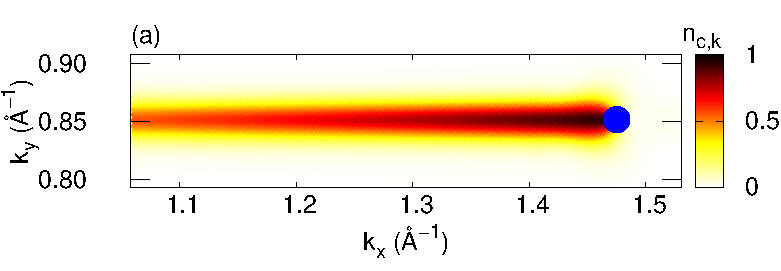
\includegraphics[width=0.8\linewidth]{pic/pop_dist.pdf}
	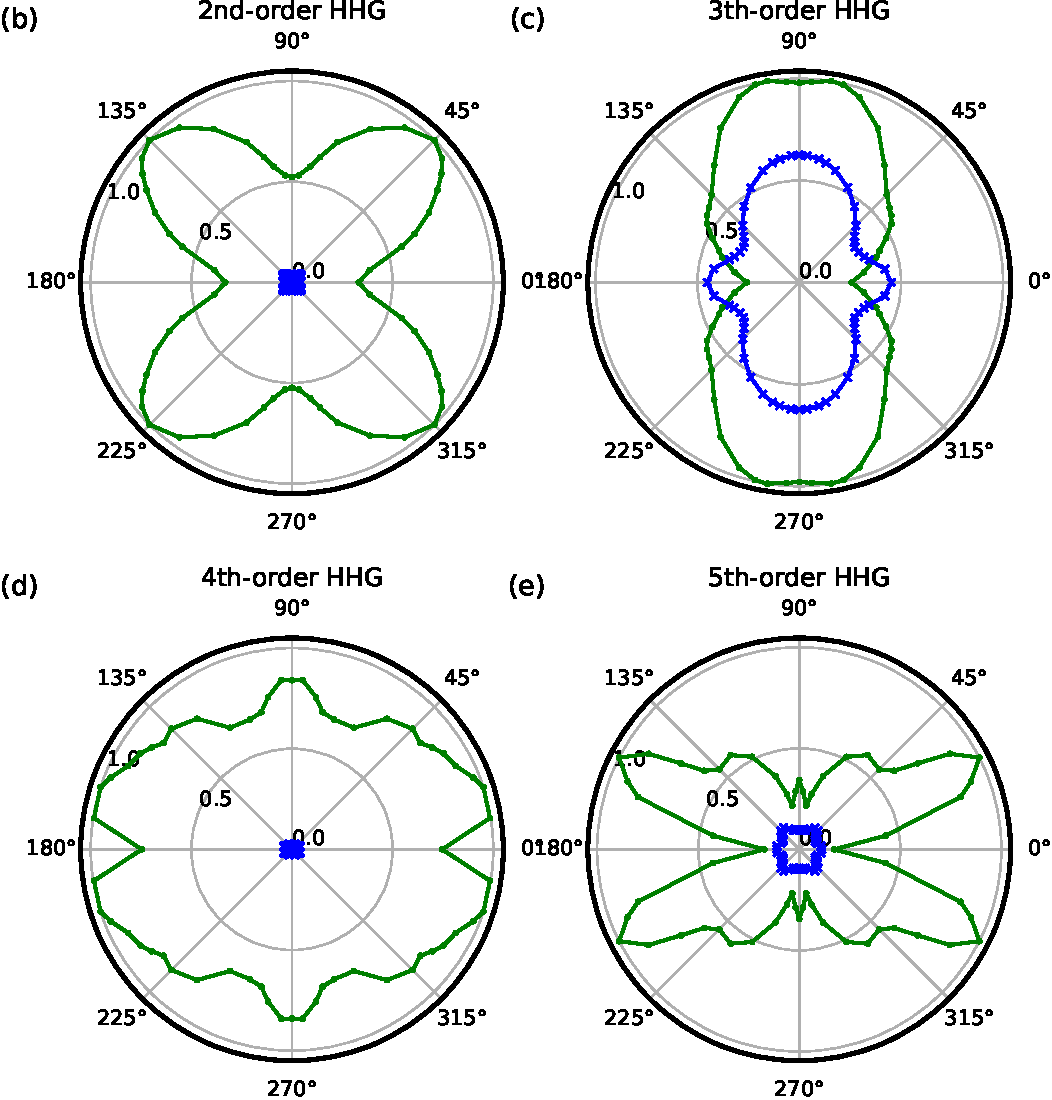
\includegraphics[width=0.8\linewidth]{pic/pop_c.pdf}
	\caption{\label{fig:pop}
		(a) The calculated conduction population distribution, $n^{\mathrm{neq-steady}}_{c\mathbf k}$ for the nonequilibrium steady-state is shown. Here, the Dirac point is indicated by the blue circle. (b--e) The angular dependence of the induced harmonic intensity is shown for the (b) second, (c) third, (d) fourth, and (e) fifth harmonics. The results obtained using the nonequilibrium population model and the nonequilibrium steady-state are shown by the blue and green solid lines, respectively. Panels are reproduced with permission from ref.~(\cite{PhysRevB.109.045421}). Copyright 2024, Phys. Rev. B.
	}
\end{figure}

In our exploration of the coherent coupling between the MIR and THz fields, beyond the population contribution induced by the THz field, we introduce a nonequilibrium population distribution model as an extension of the thermodynamic model.

Within the thermodynamic model, the THz field's contribution is represented by adjusting the population distribution via an increased electronic temperature in the reference Fermi--Dirac distribution. This model captures only the population contribution, corresponding to the diagonal elements of the density matrix, based on the thermal distribution.

To look into the coherent coupling contribution, we extend the thermodynamic model by substituting the reference Fermi--Dirac distribution in the relaxation operator (Eq. (\ref{eqn:relaxation})) with the population distribution of the nonequilibrium steady state under a static field. This extension incorporates the population contribution, signified by diagonal elements of the density matrix, while omitting THz-induced coherence, represented by the off-diagonal elements of the density matrix.

By comparing the nonequilibrium population model with the fully dynamical model, which includes both population and coherence effects, we can distinguish the role of coherent coupling between the THz and MIR fields. This comparative analysis helps illustrate the distinct contributions of population and coherence effects to HHG, providing valuable insights into the underlying mechanisms governing this phenomenon.
To formulate the nonequilibrium population model, we first analyze the population distribution in the nonequilibrium steady state under a static field. The population distribution in the Brillouin zone can be expressed as
\begin{align}
	n_{b \mathbf k}(t) & = \int d \mathbf k' \delta(\mathbf k - \mathbf K'(t)) \mathrm{Tr}\left [
	| u^H_{b\mathbf k'}(t)\rangle \langle u^H_{b\mathbf k'}(t)| \rho_{\mathbf k'}(t)
	\right ] \nonumber                                                                                  \\
	                   & =\langle u^H_{b,\mathbf k-e\mathbf A(t)}(t)| \rho_{\mathbf k-e\mathbf A(t)}(t)
	| u^H_{b,\mathbf k-e\mathbf A(t)}(t)\rangle,
\end{align}
where $\mathbf K'(t)$ is the accelerated wavevector in accordance with the acceleration theorem, $\mathbf K'(t)=\mathbf k'+e\mathbf A(t)$. The population distribution in the nonequilibrium steady state can be evaluated in the long-time propagation limit under a static field $\mathbf A(t)= -\mathbf E_{dc}t$,
\begin{align}
	n^{\mathrm{neq-steady}}_{b\mathbf k} = \lim _{t\rightarrow \infty } n_{b \mathbf k}(t).
\end{align}

In Fig.\ref{fig:pop}(a), we illustrate the population distribution in the conduction band for the nonequilibrium steady-state under a static field with a strength of $E_{dc}=0.5$~MV/cm. The static field is set along the $\Gamma$--$M$ direction ($x$-axis), and the blue circle marks the Dirac point ($K$ point).

In this illustrateion, the region to the left of the Dirac point is predominantly occupied by the field-induced population in the nonequilibrium steady-state, while the region to the right of the Dirac point appears nearly empty. This asymmetry disrupts the inversion symmetry of the system. We use this nonequilibrium population distribution as the reference distribution of the relaxation operator in Eq.~(\ref{eqn:relaxation}) instead of the Fermi--Dirac distribution to establish the nonequilibrium population model.

In Fig.\ref{fig:pop}(b), we present the angular dependence of the second-harmonic  under a static field with a strength of $E_{dc}=0.5$MV/cm. The corresponding angular dependences of the third, fourth, and fifth harmonics are showned in Figs.\ref{fig:pop}(c--e), respectively. Each panel displays results obtained using the nonequilibrium population model as the blue solid line, compared with results derived from the quasi-static approximation, showned as the green solid line, which matches the result shown in Fig.\ref{fig:polar}.

Figs~\ref{fig:pop}~(b) and (d) highlight that even-order harmonics computed with the nonequilibrium population model are notably weaker compared to those calculated using the fully dynamical approach based on the quasi-static approximation. This difference indicates that under the charge-neutral condition ($\mu=0$) examined here, the resonant effects of the MIR field at two- and four-photon resonances are significantly distant from the Fermi level. Consequently, modifications to the population near the Fermi surface  minor contributions to even-order harmonic generation. In contrast, the fully dynamical calculation reveals that the THz field can coherently couple with the MIR field via off-diagonal elements of the density matrix, enabling coherent coupling not only around the Fermi level but also across the Brillouin zone wherever dipole transitions are permitted. Thus, the coherent coupling component may strengthen even-order harmonic generation by enhancing contributions from resonant quantum pathways.

Fig.\ref{fig:pop}(c) demonstrates that the third-harmonic  computed using the fully dynamical model is $1.57$ times stronger than that obtained using the nonequilibrium population model when the fields are perpendicular. This result suggests that the THz field enhances third-harmonic generation for the perpendicular configuration, with both coherent coupling and incoherent population playing crucial roles in this THz-assisted enhancement mechanism. On the other hand, when the fields are parallel, the third-harmonic  calculated using the fully dynamical approach is $0.57$ times weaker than that computed using the nonequilibrium population model. This finding indicates that contributions from coherent coupling and incoherent population act against each other, subsidingthe overall signal. Thus, both coherent coupling and incoherent population influence third-harmonic generation depending on the relative angle $\theta$ between the THz and MIR fields.

In Fig.\ref{fig:pop}(e), we observe that the fifth-order harmonic  computed using the fully dynamical model is significantly higher than that obtained using the nonequilibrium population model, except when the MIR and THz fields are parallel. This observation suggests that coherent coupling predominantly contributes to the enhancement of fifth-harmonic generation for most angles, although both coherent coupling and incoherent population effects are relevant when the fields are parallel. These consistent results are similarly observed for higher-order harmonics in Figure.~(\ref{fig:SI_pop}):
\begin{figure}[tb]
	\center
	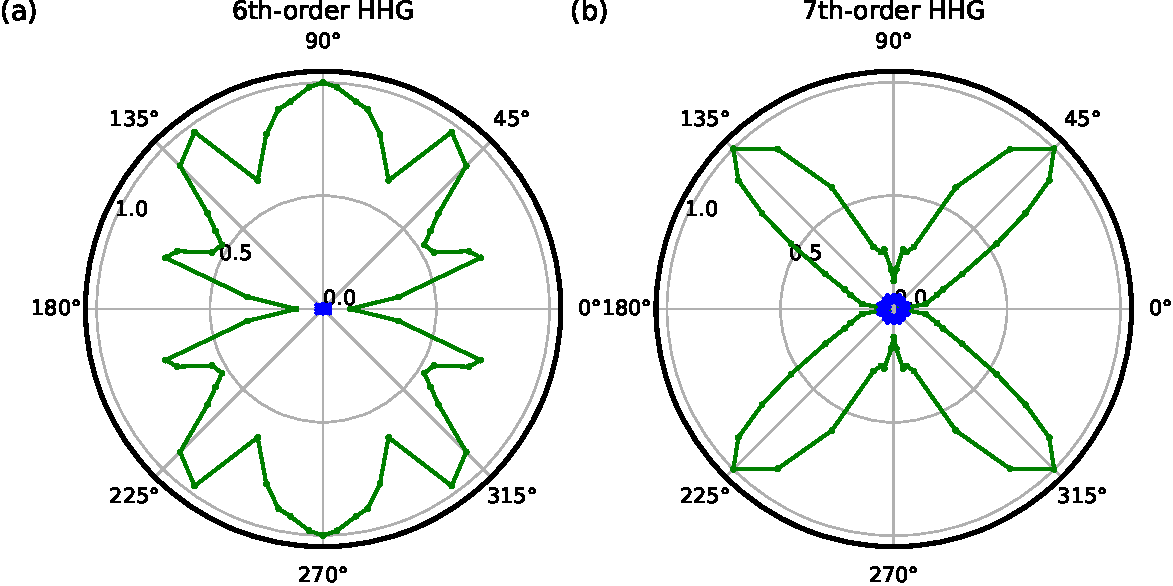
\includegraphics[width=0.8\linewidth]{pic/SI_pop.pdf}
	\caption{\label{fig:SI_pop}
		The angular dependence of the emitted harmonic intensity for the (a) sixth and (b) seventh harmonics are shown. The results obtained using the nonequilibrium population model and the nonequilibrium steady-state are shown by the blue and green solid lines, respectively. Figure is reproduced with permission from ref.~(\cite{PhysRevB.109.045421}). Copyright 2024, Phys. Rev. B.
	}
\end{figure}

We contrasted the outcomes for the sixth and seventh harmonics utilizing both the nonequilibrium population model and the nonequilibrium steady state. In Figures~\ref{fig:SI_pop}~(a) and (b), we illustrate the angular dependency of the sixth- and seventh-harmonic yields under a static field strength of $E_{dc}=0.5$MV/cm, respectively. In agreement with the analysis depicted in Fig.\ref{fig:pop}, the coherent interaction between the MIR and THz fields significantly enhances the high harmonic generation (HHG), surpassing mere field-induced population effects.
In summary, when only a MIR field is applied to graphene, the induced HHG is attributed to interference between multiple excitation pathways involving nonlinear coupling between MIR-induced intraband and interband transitions. On the other hand, the substantial enhancement of HHG observed in the presence of THz fields indicates the activation of an additional nonlinear coupling mechanism. This mechanism arises from coherent coupling between MIR- and THz-induced transitions, suggesting its predominance over other processes in contributing to overall harmonic .

The comparison between the results obtained using the fully dynamical calculation and the nonequilibrium population distribution model has provided valuable insights into the roles of coherent coupling between the MIR and THz fields. The dominance of coherent coupling in generating THz-induced even-order harmonics and enhancing high-order harmonics suggests its crucial role in driving nonlinear optical processes in solids. On the other hand, the enhancement of third harmonics under a THz field is influenced by both coherent coupling and the nonequilibrium population. Furthermore, coherent coupling appears to predominantly contribute to the enhancement of higher-order harmonics.

Importantly, these enhancement mechanisms are not limited to specific laser parameters but can be realized under more general conditions. Therefore, effective control of both coherent coupling and population dynamics becomes essential for increasing HHG from solids using multicolor laser fields.

Furthermore, the significance of coherent coupling extends across various orders of harmonic generation, as evidenced by the coherent coupling mechanism's influence on low-order harmonic phenomena (see Fig.~\ref{fig:pop}). This highlights the research necessity of field-induced coherence in nonlinear optical effects more broadly. Consequently, these findings hint at the potential for efficiently controlling electron and spin dynamics through coherent coupling, adding multi-color lasers. Such capabilities would exceed mere frequency conversion of light, opening ways for the advancement of ultrafast optoelectronics and optospintronics.
